\documentclass{article}
\usepackage{../header}
\usepackage{epigraph}
% Source - https://tex.stackexchange.com/a/760
% Posted by Vivi, modified by community. See post 'Timeline' for change history
% Retrieved 2026-06-22, License - CC BY-SA 4.0
\def\Xint#1{\mathchoice
	{\XXint\displaystyle\textstyle{#1}}%
	{\XXint\textstyle\scriptstyle{#1}}%
	{\XXint\scriptstyle\scriptscriptstyle{#1}}%
	{\XXint\scriptscriptstyle\scriptscriptstyle{#1}}%
	\!\int}
\def\XXint#1#2#3{{\setbox0=\hbox{$#1{#2#3}{\int}$ }
		\vcenter{\hbox{$#2#3$ }}\kern-0.6\wd0}}
\def\ddashint{\Xint=}
\def\dashint{\Xint-}
\setcounter{tocdepth}{4}


\title{Hyperbolic Partial Differential Equations}
\author{Aniruddha Madhava}
\date{June 2026}

\begin{document}
	
	\maketitle
	\tableofcontents 
	\halfline 
	\newpage 
	
	\part{The Wave Equation}
	\epigraph{I was observing the motion of a boat which was rapidly drawn along a narrow channel by a pair of horses, when the boat suddenly stopped—not so the mass of water in the channel which it had put in motion; it accumulated round the prow of the vessel in a state of violent agitation, then suddenly leaving it behind, rolled forward with great velocity, assuming the form of a large solitary elevation, a rounded, smooth and well-defined heap of water, which continued its course along the channel apparently without change of form or diminution of speed. I followed it on horseback, and overtook it still rolling on at a rate of some eight or nine miles an hour, preserving its original figure some thirty feet long and a foot to a foot and a half in height. Its height gradually diminished, and after a chase of one or two miles I lost it in the windings of the channel. Such, in the month of August 1834, was my first chance interview with that singular and beautiful phenomenon which I have called the Wave of Translation.}{John Scott Russell}
	
	{\huge \uline{\textbf{Resources}}:}
	{\large\begin{enumerate}[label = \arabic{*}.]
			\item \textit{Partial Differential Equations} (2nd Ed.), Lawrence C. Evans
			\item \textit{Introduction to Nonlinear Wave Equations}, Jonathan Luk
		\end{enumerate}
	}
	
	
	\newpage 
	\section{Introduction to the Wave Equation}
	\subsection{Explicit Representation Formulas}
	
	In this section, we talk will work through the derivations of explicit representation formulas for initial value problems of the \textit{wave equation},
	\begin{equation}
		\Box u\coloneqq u_{tt} - \Delta u = 0 \quad (\text{or more generally, } f), 
	\end{equation}
	where the unknown is the function $u: \bar{U} \times [0, \infty) \to \mathbb{R}$, $u = u(x, t)$, with $x \in U^{\text{open}} \subseteq \mathbb{R}^{n}$ and $t > 0$, $\Delta$ is taken with respect to the spatial variables $x = (x_{1}, \ldots, x_{n})$, and $f: U \times [0, \infty) \to \mathbb{R}$ is a given function. 
	
	\subsubsection{The Wave Equation in One Spatial Dimension -- D'Alembert's Formula}
	The simplest example of the wave equation happens in the case $n = 1$. Consider the following initial value problem, 
	\begin{equation}
		\left\{
		\begin{alignedat}{3}
			&u_{tt} - u_{xx} &= 0 &\qquad \text{ in $\mathbb{R} \times (0, \infty)$}  \\
			&u = g,  u_{t} &= h &\qquad \text{ on $\mathbb{R} \times \{t = 0\}$}. 
		\end{alignedat}
		\right.
	\end{equation}
	We note that the wave equation can be written in a more suggestive manner: 
	\begin{equation}
		0 = u_{tt} - u_{xx} = (\partial_{t} + \partial_{x})(\partial_{t} - \partial_{x})u \eqqcolon (\partial_{t} + \partial_{x})v, 
	\end{equation}
	where we set $v = v(x, t) = u_{t} - u_{x}$. Thus, $v$ satisfies the transport equation, $v_{t} + v_{x} = 0$. Using the solution to the transport equation in one dimension, one obtains the solution, 
	\begin{equation*}
		v(x, t) = a(x - t), 
	\end{equation*}
	where $a(x) \coloneqq v(x, 0)$. This gives us the nonhomogeneous transport equation, 
	\begin{equation*}
		u_{t} -u_{x} = a(x -t), 
	\end{equation*}
	for which the explicit representation formula was shown (see Appendix) to be 
	\begin{equation}
		u(x, t) = \int_{0}^{t}a(x + (t - s)- s)\;ds + g(x + t) = \frac{1}{2}\int_{x - t}^{x + t}a(y)\;dy + g(x + t). 
	\end{equation}
	It remains for us to identify the function $a(x, t)$. Using the definition of $v(x, t)$, at $t = 0$, one has, 
	\begin{equation*}
		a(x) = v(x,0) = u_{t}(x, 0) - u_{x}(x, 0) = h(x) - g'(x). 
	\end{equation*}
	Therefore, using the fundamental theorem of calculus and the above results, we conclude that 
	\begin{equation}
		\boxed{u(x, t) = \frac{1}{2}\left[g(x + t) - g(x - t)\right] + \frac{1}{2}\int_{x - t}^{x + t}h(y)\;dy} \qquad (x \in \mathbb{R}^{n}, t \geq 0). 
	\end{equation}
	This explicit formula is called \textbf{d'Alembert's formula} for $n = 1$. Hence, we have shown that \textit{if} the wave equation has a ``sufficiently smooth solution $u$'', then it must be given by d'Alembert's formula. The following theorem formalizes this result. 
	
	\begin{theorem}[Solution to the Wave Equation ($n = 1$)]
		Assume $g \in C^{2}(\mathbb{R})$, $h \in C^{1}(\mathbb{R})$, and define $u$ by d'Alembert's formula. Then \vspace{-0.25cm}
		\begin{enumerate}[itemsep =-2pt,label = (\roman{*})]
			\item $u \in C^{2}(\mathbb{R} \times [0, \infty))$. 
			\item $u_{tt} - u_{xx} = 0$ in $\mathbb{R} \times (0, \infty)$ 
			\item $\lim\limits_{\substack{(x, t) \to (x^{0}, 0) \\ t > 0}}u(x, t) = g(x^{0})$ and $\lim\limits_{\substack{(x, t) \to (x^{0}, 0) \\ t > 0}}u_{t}(x, t) = h(x^{0})$ for each point $x^{0} \in \mathbb{R}$. 
		\end{enumerate}
	\end{theorem}
	\newpage 
	\begin{proof}
		$ $\newline \vspace{-0.65cm}
		\begin{enumerate}[itemsep =-2pt,label = (\roman{*})]
			\item Define $u$ by d'Alembert's formula. Then we compute the following: 
			\begin{align*}
				\begin{split}
					u_{x} &= \frac{1}{2}[g'(x + t) + g'(x - t)] + \frac{1}{2}[h(x + t) - h(x - t)]. \\
					u_{t} &= \frac{1}{2}[g'(x + t) -g'(x - t)] + \frac{1}{2}[h(x + t) + h(x - t)], 
				\end{split}
			\end{align*}
			whence 
			\begin{align*}
				\begin{split}
					u_{xx} &= \frac{1}{2}[g''(x + t) + g''(x - t)] + \frac{1}{2}[h'(x + t) - h'(x - t)]. \\ 
					u_{xt} &= \frac{1}{2}[g''(x + t) - g''(x - t)] + \frac{1}{2}[h'(x + t) + h'(x - t)].  \\
					u_{tt} &= \frac{1}{2}[g''(x + t) +  g''(x - t)] + \frac{1}{2}[h'(x + t) - h'(x - t)]. 
				\end{split}
			\end{align*}
			Since $g', g''$ and $h, h'$ are all continuous at every $x \in \mathbb{R}$ and $t \in [0, \infty)$, as are the functions $x + t$ and $x - t$, we conclude that each of the first and second-order partial derivatives of $u$ are continuous on $\mathbb{R} \times [0, \infty)$. Thus, $u \in C^{2}(\mathbb{R} \times [0,\infty))$. 
			\item From the above calculations, it follows immediately that $u_{tt} - u_{xx} = 0$. 
			\item By (1), $u$ is continuous at every $(x, t) \in \mathbb{R} \times [0, \infty)$, and thus continuous at every point of the form $(x^{0}, 0) \in \mathbb{R} \times \{0\}$. Thus by the limit definition of continuity, one has 
			\begin{equation*}
				\lim_{(x, t) \to (x^{0}, 0)}u(x, t) = u(x^{0}, 0) \eqqcolon g(x^{0}). 
			\end{equation*}
			Likewise, by our remark above, $u_{t}(x, t) \in C^{1}(\mathbb{R} \times [0, \infty)$. Thus by the limit definition of continuity, one has 
			\begin{equation*}
				\lim_{(x, t) \to (x^{0}, 0)} u_{t}(x, t) = u_{t}(x^{0}, 0) \eqqcolon h(x^{0}). 
			\end{equation*}
		\end{enumerate}
	\end{proof}
	
	\subsubsection{The Wave Equation in One Spatial Dimension -- Half-Line}
	Now we will consider the modified initial value problem, 
	\begin{equation}
		\left\{
		\begin{alignedat}{3}
			&u_{tt} - u_{xx} &=0 &\qquad (\text{in $\mathbb{R}_{+} \times (0, \infty)$} \\
			&u = g, u_{t} &=h &\qquad (\text{in $\mathbb{R}_{+} \times \{t = 0\}$}) \\
			&u = 0 & &\qquad (\text{on $\{x = 0\} \times (0,\infty)$}. 
		\end{alignedat}
		\right.
	\end{equation}
	To solve this problem, we will use the \textit{method of reflections}; i.e., we will extend the initial value problem to the entire real line by means of the odd reflections: 
	\begin{equation*}
		\ti{u}(x, t) = 
		\begin{cases}
			u(x, t) & x \geq 0 \\
			-u(-x,t) & x \leq 0.  
		\end{cases}
	\end{equation*}
	\begin{equation*}
		\ti{g}(x) = 
		\begin{cases}
			g(x), & x \geq 0 \\
			-g(-x), & x \leq 0,
		\end{cases}
	\end{equation*}
	\begin{equation*}
		\ti{h}(x) = 
		\begin{cases}
			h(x), & x \geq 0 \\
			-h(-x), & x \leq 0. 
		\end{cases}
	\end{equation*}
	It is straightforward to check that $\ti{u}, \ti{g}, \ti{h}$ satisfy the ordinary wave equation ($n= 1$) on the whole real line. Thus by d'Alembert's formula, we obtain the following solution: 
	\begin{equation}
		\boxed{u(x, t) = 
			\left\{
			\begin{alignedat}{2}
				&\frac{1}{2}[g(x + t) - g(x-t)] + \frac{1}{2}\int_{x -t}^{x + t}h(y)\;dy &\qquad (x\geq t \geq 0)\\
				&\frac{1}{2}[g(x + t) - g(t - x)] + \frac{1}{2}\int_{t - x}^{x + t}h(y)\;dy &\qquad (0 \leq x \leq t)
			\end{alignedat}
			\right.
		}
	\end{equation}
	
	\subsubsection{The Wave Equation in \texorpdfstring{$n\geq 2$}{>2} Spatial Dimension -- Kirchoff's and Poisson's Formulas}
	In this subsection, we will develop explicit representation formulas for the wave equation for dimensions $n \geq 2$. To develop these formulas, we require the \textit{method of spherical means}. Consider the following definitions. 
	
	\begin{definition}[Spherical Means]
		$ $\newline \vspace{-0.25cm}
		\begin{enumerate}[itemsep =-2pt,label = (\roman{*})]
			\item Let $x \in \mathbb{R}^{n}$, $t > 0$, and $r > 0$. We define the average of $u(\cdot, t)$ over the sphere $\partial B(x, r)$ to be 
			\begin{equation}
				U(x;r, t) = \dashint_{\partial B(x, r)} u(y,t)\;dS(y).
			\end{equation}
			\item We make the analogous definitions, 
			\begin{equation}
				\begin{cases}
					G(x; r) &= \dashint_{\partial B(x,r)}g(y)\;dS(y). \\
					H(x; r) &= \dashint_{\partial B(x,r)}h(y)\;dS(y). 
				\end{cases}
			\end{equation}
		\end{enumerate}
		For any fixed $x$, we will regard $U, G, H$ as functions of $r$ and $t$. 
	\end{definition}
	
	\begin{lemma}[Euler-Poisson-Darboux Equation]
		Fix $x \in\mathbb{R}^{n}$, $n, m \geq 2$, and let $u \in C^{m}(\mathbb{R}^{n} \times [0, \infty))$ satisfy the initial value problem, 
		\begin{equation*}
			\left\{
			\begin{alignedat}{3}
				&u_{tt} - \Delta u &= 0 &\qquad (\text{in $\mathbb{R}^{n} \times (0,\infty)$}) \\
				&u = g, u_{t} &= h &\qquad (\text{in $\mathbb{R}^{n} \times \{t = 0\}$}). 
			\end{alignedat}
			\right. 
		\end{equation*}
		Then $U \in C^{m}(\overline{\mathbb{R}}_{+} \times [0,\infty))$, and $U_{tt}$ satisfies the \textit{Euler-Poisson-Darboux} initial value problem, 
		\begin{equation}
			\left\{
			\begin{alignedat}{3}
				&U_{tt} - U_{rr} - \frac{n-1}{r}U_{r} &= 0 & \qquad (\text{in $\mathbb{R}_{+} \times (0,\infty)$)} \\
				&U = G, U_{t} = H& &\qquad (\text{on $\mathbb{R}_{+} \times \{t = 0\}$}
			\end{alignedat}
			\right. 
		\end{equation}
	\end{lemma}
	\begin{proof}
		We begin by taking the partial derivative of the spherical mean $U$ with respect to $r$. To do so, we rewrite 
		\begin{equation*}
			U(x;r,t) = \dashint_{\partial B(x, r)}u(y,t)\;dS(y) = \frac{1}{n\alpha(n)r^{n-1}}\int_{\partial B(x, r)}u(y,t)\;dS(y) = \frac{1}{n\alpha(n)}\int_{\partial B(0,1)}u(x + rz, t)\;dS(z). 
		\end{equation*}
		Thus, 
		\begin{align*}
			\begin{split}
				U_{r}(x;r, t) &= \frac{1}{n\alpha(n)}\frac{\partial}{\partial r}\int_{\partial B(0,1)}u(x + rz, t)\;dS(z) \\
				&= \frac{1}{n\alpha(n)}\int_{\partial B(0,1)}Du(x + rz, t) \cdot z \;dS(z) \\
				&= \frac{r^{1-n}}{n\alpha(n)}\int_{\partial B(x, r)}Du(y, t) \cdot \frac{y -x}{r}\;dS(y) \\
				&= \frac{r}{n\alpha(n)r^{n}}\int_{\partial B(x, r)}\frac{\partial u}{\partial \nu}\;dS(y) \\
				&= \frac{r}{n\alpha(n)r^{n}}\int_{B(x, r)}\Delta u\;dy = \frac{r}{n}\dashint_{B(x, r)}\Delta u\;dy,
			\end{split}
		\end{align*}
		where passing the derivative inside the integral in the second line is justified since $u$ is sufficiently smooth (meaning that $Du$ exists a.e. and is integrable on $\partial B(0,1)$), and the final line follows from Green's formula. Now taking some large $R > 0$, and restricting to $0 < r \leq R/2$, one has that since $B(x,r) \subset \overline{B(x, R/2)}$ and $\Delta u$ is continuous (so that the extreme value theorem applies), 
		\begin{equation*}
			\norm{\Delta u}_{L^{\infty}(B(x, r))} \leq \norm{\Delta u}_{L^{\infty}(B(x, R))} \eqqcolon C < \infty. 
		\end{equation*}
		Hence, 
		\begin{equation*}
			U_{r}(x;r, t) \leq \frac{C}{n}r \implies \lim_{r \to 0^{+}}U_{r}(x;r, t) = 0.
		\end{equation*}
		Now we will compute the second partial derivative of $U$ with respect to $r$. We compute, 
		\begin{align*}
			\begin{split}
				U_{rr}(x;r, t) &= \frac{1 -n}{n\alpha(n)r^{n}}\int_{B(x, r)}\Delta u\;dy + \frac{r^{1-n}}{n\alpha(n)}\frac{\partial}{\partial r}\int_{B(x, r)}\Delta u(y,t)\;dy \\
				&= \frac{1 - n}{n}\dashint_{B(x, r)}\Delta u(y,t)\;dy + \frac{r^{1-n}}{n\alpha(n)}\int_{\partial B(x, r)}\Delta u(y,t)\;dS(y) \\
				&= \dashint_{\partial B(x, r)}\Delta u(y, t)\;dS(y) + \left(\frac{1}{n} - 1\right)\dashint_{B(x, r)}\Delta u(y, t)\;dy, 
			\end{split}
		\end{align*}
		where the second line follows from the coarea formula (see Appendix). By applying similar reasoning to above, one computes that $\lim_{r \to 0^{+}}U_{rr}(x;r, t) = (1/n)\Delta u$. In this manner, repeatedly differentiating $U$, one sees that $U \in C^{m}(\overline{\mathbb{R}}_{+} \times [0, \infty))$. Now differentiating, 
		\begin{align*}
			\begin{split}
				(n-1)r^{n - 2}U_{r} + r^{n-1}U_{rr} &= \frac{d}{dr}(r^{n-1}U_{r}) \\
				&= \frac{d}{dr}\frac{1}{n\alpha(n)}\int_{B(x,r)}u_{tt}\;dy  \\
				&= \frac{1}{n\alpha(n)}\int_{\partial B(x,r)}u_{tt}\;dS(y)  \\
				&= r^{n-1}\dashint_{\partial B(x, r)}u_{tt}\;dS(y) \eqqcolon r^{n-1}U_{tt}, 
			\end{split}
		\end{align*}
		with the third line following from the coarea formula. 
	\end{proof}
	
	Now we will derive the explicit representation formula for the 3-dimensional wave equation by reducing the system to the one-dimensional Euler-Poisson-Darboux equation and solving this system using the formula we derived for the one-dimensional half-line equation. 
	
	\paragraph{Kirchoff's Formula for the Wave Equation \texorpdfstring{($n = 3$)}{n =3}}
	Suppose $u \in C^{2}(\mathbb{R}^{3} \times [0,\infty))$ solves the initial-value problem 
	\begin{equation}
		\left\{
		\begin{alignedat}{3}
			&u_{tt} - \Delta u &= 0 &\qquad (\text{in $\mathbb{R}^{3} \times [0,\infty)$}) \\
			&u = g, u_{t} &=h &\qquad (\text{on $\mathbb{R}^{3} \times \{t = 0\}$})
		\end{alignedat}
		\right.
	\end{equation}
	Define the functions, $\ti{U} = rU(x;r, t)$, $\ti{G}(r) = rG(x;r)$, and $\ti{H}(r) = rH(x;r)$. Then we observe the following: 
	\begin{enumerate}[itemsep =-2pt, label = (\roman{*})]
		\item $ $\newline \vspace{-0.75cm}
		\begin{align*}
			\begin{split}
				\ti{U}_{tt} &= rU_{tt} = r\left[U_{rr} + \frac{2}{r}U_{r}\right] \\
				&= rU_{rr} + 2U_{r} = (U + rU_{r})_{r} = \ti{U}_{rr}. 
			\end{split}
		\end{align*}
		\item On $\mathbb{R}_{+} \times \{t = 0\}$, $U = G$ and $U_{t} = H$ so that $\ti{U} =\ti{G}$ and $\ti{U}_{t} = \ti{H}$. 
		\item For $r = 0$, $\partial B(x, 0) = \varnothing$ so that $\ti{U} = 0$ on $\{r = 0\} \times (0, \infty)$. 
	\end{enumerate}
	In other words, we have shown that $\ti{U}$ satisfies the following initial value problem, 
	\begin{equation*}
		\left\{
		\begin{alignedat}{3}
			&\ti{U}_{tt} - \ti{U}_{rr} &= 0 &\qquad (\text{in $\mathbb{R}_{+} \times (0,\infty)$}) \\
			&\ti{U} = \ti{G}, \ti{U}_{t} &= \ti{H} &\qquad (\text{on $\mathbb{R}_{+} \times \{t = 0\}$}) \\
			&\ti{U} = 0 &&\qquad (\text{on $\{r = 0\} \times (0,\infty)$})
		\end{alignedat}
		\right.
	\end{equation*}
	Using the solution for the one-dimensional wave equation on the half-line, for $0 \leq r \leq t$, one has 
	\begin{equation*}
		\ti{U}(x; r, t) = \frac{1}{2}[\ti{G}(r + t) - \ti{G}(t - r)] + \frac{1}{2}\int_{t -r}^{r + t}\ti{H}(y)\;dy. 
	\end{equation*}
	On the other hand, one has that 
	\begin{align*}
		\begin{split}
			u(x, t) &= \lim_{r \to 0^{+}}\frac{\ti{U}(x; r, t)}{r} \\
			&= \lim_{r \to 0^{+}}\left[\frac{\ti{G}(r + t) - \ti{G}(t - r)}{2r} + \frac{1}{2r}\int_{t - r}^{r + t}\ti{H}(y)\;dy\right] \\
			&= \ti{G}'(t) + \ti{H}(t). 
		\end{split}
	\end{align*}
	Recall again that 
	\begin{align}
		\begin{split}
			\ti{G}'(t) &= \frac{\partial}{\partial t}\left(t\dashint_{\partial B(x, t)}g(y)\;dS(y)\right) \\
			&= \frac{\partial}{\partial t}\left(\frac{1}{n\alpha(n)t}\int_{\partial B(x ,t)}g(y)\;dS(y)\right) \\
			&= -\frac{1}{n\alpha(n)t^{2}}\int_{\partial B(x,t)}g(y)\;dS(y) + \frac{1}{n\alpha(n)t}\frac{\partial}{\partial t}\left(t^{2}\int_{\partial B(0,1)}g(x + tz)\;dS(z)\right) \\
			&= -\dashint_{\partial B(x, t)}g(y)\;dS(y) + \frac{2}{n\alpha(n)}\int_{\partial B(0,1)}g(x + tz)\;dS(z) + \frac{1}{n\alpha(n)t}\int_{\partial B(x, t)}Dg(y) \cdot \left(\frac{y - x}{t}\right)\;dS(y) \\
			&= \dashint_{\partial B(x, t)}g(y)\;dS(y) + \dashint_{\partial B(x, t)}Dg(y) \cdot (y - x)\;dS(y). 
		\end{split}
	\end{align}
	Likewise, one has 
	\begin{equation*}
		\ti{H}(t) = tH(t) = \dashint_{\partial B(x, t)}th(y)\;dS(y). 
	\end{equation*}
	Therefore, we conclude that 
	\begin{equation}
		\boxed{u(x, t) = \dashint_{\partial B(x, t)}th(y) + g(y) + Dg(y) \cdot (y - x)\;dS(y)}\label{eq:Kirchoff}
	\end{equation}
	This is \textbf{Kirchoff's formula} for the wave equation in dimension 3.
	
	\paragraph{Poisson's Formula for the Wave Equation \texorpdfstring{($n = 2$)}{n=2}} Assume $u \in C^{2}(\mathbb{R}^{2} \times [0,\infty))$ solves the IVP for $n = 2$. Unlike for the $n = 3$ case, we will consider the 2-dimensional problem and ``view'' it as a 3-dimensional problem. Define $\bar{u}(x_{1}, x_{2}, x_{3}, t) = u(x_{1}, x_{2}, t)$ so that $u$ satisfies the IVP 
	\begin{equation*}
		\left\{
		\begin{alignedat}{3}
			&\bar{u}_{tt} - \Delta \bar{u} &= 0 &\qquad(\text{in $\mathbb{R}^{3} \times (0, \infty)$}) \\
			&\bar{u} =\bar{g}, \bar{u}_{t} &= \bar{h} &\qquad(\text{on $\mathbb{R}^{3} \times \{t = 0\}$}), 
		\end{alignedat}
		\right.
	\end{equation*}
	where we define $\bar{g}$ and $\bar{h}$ analogously. For $x = (x_{1}, x_{2}) \in \mathbb{R}^{2}$, write $\bar{x} = (x_{1}, x_{2}, 0) \in \mathbb{R}^{3}$. Then by Kirchoff's formula, one has 
	\begin{equation*}
		u(x, t) = \bar{u}(\bar{x}, t) = \frac{\partial}{\partial t}\left(t\dashint_{\partial \bar{B}(\bar{x},t)}\bar{g}d\bar{S}\right) + t\dashint_{\partial \bar{B}(\bar{x},t)}\bar{h}d\bar{S}, 
	\end{equation*}
	where $\bar{B}(\bar{x}, t)$ denotes the ball in $\mathbb{R}^{3}$ with center $\bar{x}$, radius $t > 0$, and where $d\bar{S}$ denotes the 2-dimensional surface measure on $\partial \bar{B}(\bar{x}, t)$. But we can write 
	\begin{equation*}
		\dashint_{\partial \bar{B}(\bar{x},t)}\bar{g}d\bar{S} = \frac{1}{4\pi t^{2}}\int_{\partial \bar{B}(\bar{x}, t)}\bar{g}d\bar{S} = \frac{2}{4\pi t^{2}}\int_{B(x,t)}g(y)(1 + |D\gamma(y)|^{2})^{1/2}\;dy, 
	\end{equation*}
	where $\gamma(y) = (t^{2} - |y - x|^{2})^{1/2}$ for $y \in B(x, t)$. The factor 2 comes from the two hemispheres of $\partial\bar{B}(\bar{x}, t)$. Since $(1 + |D\gamma|^{2})^{1/2} = t(t^{2} - |y - x|^{2})^{-1/2}$, one has 
	\begin{align*}
		\begin{split}
			\dashint_{\partial \bar{B}(\bar{x}, t)}\bar{g}d\bar{S} &= \frac{1}{2\pi t}\int_{B(x,t)}\frac{g(y)}{(t^{2} - |y - x|^{2})^{1/2}}\;dy \\
			&= \frac{t}{2}\dashint_{B(x,t)}\frac{g(y)}{(t^{2} - |y - x|^{2})^{1/2}}\;dy.
		\end{split}
	\end{align*}
	Using this and the coarea formula, one obtains 
	\begin{equation*}
		u(x, t) = \frac{1}{2}\frac{\partial}{\partial t}\left(t^{2}\dashint_{B(x,t)}\frac{g(y)}{(t^{2} - |y - x|^{2})^{1/2}}\;dy\right) + \frac{t^{2}}{2}\dashint_{B(x,t)}\frac{h(y)}{(t^{2} - |y - x|^{2})^{1/2}}\;dy.
	\end{equation*}
	Using the same reasoning as above to pass the derivative inside the integral, one has 
	\begin{align*}
		\begin{split}
			\frac{\partial}{\partial t}\left(t^{2}\dashint_{B(x,t)}\frac{g(y)}{(t^{2} - |y - x|^{2})^{1/2}}\;dy\right) &= t\dashint_{B(x,t)}\frac{g(y)}{(t^{2} - |y - x|^{2})^{1/2}}\;dy + t\dashint_{B(x,t)}\frac{Dg(y) \cdot (y -x)}{(t^{2} - |y - x|^{2})^{1/2}}\;dy. 
		\end{split}
	\end{align*}
	Thus for $n = 2$, we obtain \textbf{Poisson's Formula}, 
	\begin{equation}
		\boxed{
			u(x,t) = \frac{1}{2}\dashint_{B(x,t)}\frac{ tg(y) + t^{2}h(y) + tDg(y) \cdot (y -x) }{(t^{2} - |y - x|^{2})^{1/2}}\;dy \qquad \quad (x \in \mathbb{R}^{2}, t > 0)
		}
	\end{equation}
	Notice that in solving the wave equation for $n = 2$, we used the \textit{method of descent}; i.e., we solved the problem for $n = 3$ first, and then dropped down to $n =2$. 
	
	\paragraph{General Solutions for \texorpdfstring{$n\geq 2$}{n > 1}} Following similar extensive calculations as above (see Appendix for the work), we obtain the following solutions to the wave equation, 
	\begin{equation}
		\boxed{
			u(x, t) = 
			\left\{
			\begin{alignedat}{2}
				&\frac{1}{\gamma(n)}\left[\left(\frac{\partial}{\partial t}\right)\left(\frac{1}{t}\frac{\partial}{\partial t}\right)^{\frac{n-3}{2}}\left(t^{n-2}\dashint_{\partial B(x,t)}g\;dS\right) + \left(\frac{1}{t}\frac{\partial}{\partial t}\right)^{\frac{n-3}{2}}\left(t^{n-2}\dashint_{\partial B(x,t)}h\;dS\right)\right] &\qquad \substack{\displaystyle n \geq 3 \\ \displaystyle n \text{ odd}} \\
				&\frac{1}{\beta(n)}\left[\left(\frac{\partial}{\partial t}\right)\left(\frac{1}{t}\frac{\partial}{\partial t}\right)^{\frac{n-2}{2}}\left(t^{n}\dashint_{B(x,t)}\frac{g(y)}{(t^{2} - |y - x|^{2})^{1/2}}\;dy\right)\right. &\\
				&\qquad \qquad \qquad \left.+ \left(\frac{1}{t}\frac{\partial}{\partial t}\right)^{\frac{n-2}{2}}\left(t^{n}\dashint_{B(x,t)}\frac{h(y)}{(t^{2} - |y - x|^{2})^{1/2}}\;dy\right)\right] &\qquad \substack{\displaystyle n \geq 2 \\ \displaystyle n \text{ even}}
			\end{alignedat}
			\right.
		}
	\end{equation}
	where in the first equation $\gamma_{n} = 1 \cdot 3 \cdot \dotsm\cdot (n-2)$, and $\beta(n) = 2 \cdot 4 \cdot \dotsm \cdot (n-2) \cdot n$. The above solutions highlight an interesting contrast between odd-dimensional, and even-dimensional solutions. Note that if $n$ is odd and $n \geq 3$, the initial data at a point $x\in \mathbb{R}^{n}$ only affect the solution $u$ along the boundary $\{(y,t) \mid t > 0, |x -y| = t\}$ of the cone $C = \{(y,t)\mid t > 0, |x - y| < t\}$. On the other hand, if $n$ is given, the initial data can affect the solution within all of $C$. Thus, a disturbance originating at $x$ propagates along a sharp wavefront in odd dimensions, but continues to have effects even after the leading edge of the wavefront passes in even dimensions. This phenomenon is \textbf{Huygen's principle}. 
	
	\subsection{Solution to the Nonomgeneous Wave Equation}
	Now we will use the solutions from the previous sections to address the nonhomogeneous wave equation, 
	\begin{equation}
		\left\{
		\begin{alignedat}{3}
			&u_{tt} - \Delta u &= f &\qquad (\text{in $\mathbb{R}^{n} \times (0,\infty)$}) \\
			&u =0, u_{t} &= 0 &\qquad (\text{on $\mathbb{R}^{n} \times \{t = 0\}$}). 
		\end{alignedat}
		\right.
	\end{equation}
	To solve this problem, we use Duhamel's principle\footnote{See \href{https://en.wikipedia.org/wiki/Duhamel\%27s\_principle}{https://en.wikipedia.org/wiki/Duhamel\%27s\_principle} for an explanation.} by setting $u = u(x,t;s)$ to be the solution of 
	\begin{equation}
		\left\{
		\begin{alignedat}{3}
			&u_{tt}(\cdot; s)- \Delta u(\cdot, s) &= 0 \qquad &(\text{in $\mathbb{R}^{n} \times (0,\infty)$}) \\
			&u(\cdot;s) =0, u_{t}(\cdot;s) &= f(\cdot,s) \qquad &(\text{on $\mathbb{R}^{n} \times \{t = 0\}$}). 
		\end{alignedat}
		\right.
	\end{equation}
	Thus, by Duhamel's principle, 
	\begin{equation}
		u(x, t) \coloneqq \int_{0}^{t}u(x,t;s)\;ds \qquad (x \in \mathbb{R}^n, t \geq 0)
	\end{equation}
	is a solution of the above nonhomogeneous wave equation. Consequently, the solution to the general inhomogeneous wave problem, 
	\begin{equation}
		\left\{
		\begin{alignedat}{3}
			&u_{tt} - \Delta u &= f &\qquad(\text{in $\mathbb{R}^n \times (0,\infty)$}) \\
			&u = g, u_t &=h &\qquad (\text{on $\mathbb{R}^n \times \{t = 0\}$})
		\end{alignedat}
		\right.
	\end{equation}
	is equal to the sum of the solutions to the problems
	\begin{equation}
		\left\{
		\begin{alignedat}{3}
			&u_{tt} - \Delta u &= 0 &\qquad(\text{in $\mathbb{R}^n \times (0,\infty)$}) \\
			&u = g, u_t &=h &\qquad (\text{on $\mathbb{R}^n \times \{t = 0\}$})
		\end{alignedat}
		\right.
		\quad 
		\text{and} 
		\quad 
		\left\{
		\begin{alignedat}{3}
			&u_{tt} - \Delta u &= f &\qquad(\text{in $\mathbb{R}^n \times (0,\infty)$}) \\
			&u = 0, u_t &=0 &\qquad (\text{on $\mathbb{R}^n \times \{t = 0\}$})
		\end{alignedat}
		\right.
	\end{equation}
	
	\subsubsection{Example 1: Solution to Nonhomogeneous Problem for \texorpdfstring{$n = 1$}{n=1}}
	By d'Alembert's formula, one has 
	\begin{equation*}
		u(x,t;s) = \frac{1}{2}\int_{x -t + s}^{x + t + s}f(y,s)\;dy. 
	\end{equation*}
	Thus, 
	\begin{equation*}
		u(x,t) = \frac{1}{2}\int_{0}^{t}\int_{x - t + s}^{x + t + s}f(y,s)\;dyds = \frac{1}{2}\int_0^t\int_{x - s}^{x + s}f(y,t-s)\;dyds \qquad (x \in \mathbb{R}, t \geq 0).
	\end{equation*}
	
	\subsubsection{Example 2: Solution to Nonhomogeneous Problem for \texorpdfstring{$n = 3$}{n=3}}
	
	By Kirchoff's formula, one has 
	\begin{equation*}
		u(x,t;s) = (t-s)\dashint_{\partial B(x,t -s)}f(y,s)\;dS. 
	\end{equation*}
	This implies that 
	\begin{align*}
		\begin{split}
			u(x, t) &= \int_{0}^{t}(t - s)\dashint_{\partial B(x, t -s)}f(y,s)\;dSds \\
			&= \int_{0}^{t}(t - s)\frac{1}{4\pi(t - s)^{2}}\int_{\partial B(x, t - s)}f(y,s)\;dSds \\
			&= \frac{1}{4\pi}\int_{0}^{t}\int_{\partial B(x, t -s)}\frac{f(y,s)}{t - s}\;dSds \\
			&= \frac{1}{4\pi}\int_{0}^{t}\int_{\partial B(x,r)}\frac{f(y, t - r)}{r}\;dSdr. 
		\end{split}
	\end{align*}
	Hence, we conclude that 
	\begin{equation*}
		u(x,t) = \frac{1}{4\pi}\int_{B(x,t)}\frac{f(y, t - |y - x|)}{|y - x|}\;dy \qquad (x \in \mathbb{R}^3, t \geq 0), 
	\end{equation*}
	where the integrand on the right is called a \textit{retarded potential}. 
	
	\subsection{An Introduction to Energy Estimates}
	
	In this section, we will introduce the concept of \textit{energy} for the initial value problems for the wave equation. Subsequently, we will use the energy to establish some fundamental properties of solutions to the wave equation. In particular, we will show uniqueness of solution, and finite propagation speed. Our standing notation for this section is as follows. We will be working with a bounded, open subset $U \subset \mathbb{R}^n$ with a smooth boundary $\partial U$, and the sets $U_{T} = U \times (0,T]$, $\Gamma_t = \bar{U}_t \setminus U_{T}$, where $T > 0$. We will also be looking at the general initial value problem, 
	\begin{equation}
		\left\{
		\begin{alignedat}{3}
			&u_tt - &\Delta u = f \qquad &\text{in $U_T$} \\
			&\quad &u = g \qquad &\text{on $\Gamma_T$} \\
			&\quad &u_t = h \qquad &\text{on $U \times \{t = 0\}$}. 
		\end{alignedat}
		\right. 
		\label{eq:gen_wave_eqn}
	\end{equation} 
	
	\begin{theorem}[Uniqueness for the Wave Equation]
		There exists at most one function $u \in C^2(\bar{U}_t)$ solving (\ref{eq:gen_wave_eqn}). 
	\end{theorem}
	\begin{proof}
		Suppose $\ti{u}$ is another solution in $C^{2}(\bar{U}_t)$ to the given initial value problem. Then $w \coloneqq u - \ti{u}$ solves the following initial value problem 
		\begin{equation*}
			\left\{
			\begin{alignedat}{3}
				&w_{tt} - &\Delta w  = 0 \qquad &\text{in $U_T$} \\
				&\quad &w = 0 \qquad &\text{on $\Gamma_T$} \\
				&\quad &w_t = 0 \qquad &\text{on $U \times \{t = 0\}$}. 
			\end{alignedat}
			\right.
		\end{equation*} 
		Define the energy, 
		\begin{equation*}
			e(t) \coloneqq \frac{1}{2}\int_{U}w_t^2(x,t) + |Dw(x,t)|^2\;dx \qquad (0 \leq t \leq T). 
		\end{equation*}
		Since $U$ was assumed to be a bounded set, and $w \in C^{2}(\bar{U}_{T})$, for all $0 \leq t \leq T$, there exist constants $M$ and $N$ so that for all $x \in U$, $|w_t(x,t)|^2 \leq M\chi_U$ and $|Dw(x,t)|^2 \leq N\chi_{U}$, both which are integrable functions since $U$ is bounded. Thus by the Dominated Convergence Theorem, when differentiating $e(t)$ with respect to $t$, we can pass the time derivative inside the integral sign to obtain the following: 
		\begin{align*}
			\begin{split}
				\dot{e}(t) &= \int_{U}w_tw_{tt} + Dw(x,t) \cdot Dw_t(x,t)\;dx \\
				&= \int_U w_t(w_{tt} - \Delta w)\;dx = 0. 
			\end{split}
		\end{align*}
		Note that there is no boundary term since $w = 0$, which means $w_t = 0$, on $\partial U \times [0, T]$. Therefore, for all $0 \leq t \leq T$, $e(t) = e(0) =0$, so that $w_t, Dw \equiv 0$ within $U_T$. Since $w \equiv 0$ on $U \times \{t = 0\}$, we conclude that $w = u - \ti{u} \equiv 0$ in $U_T$. The proof concludes. 
	\end{proof}
	\begin{figure}[t!]
		\centering
		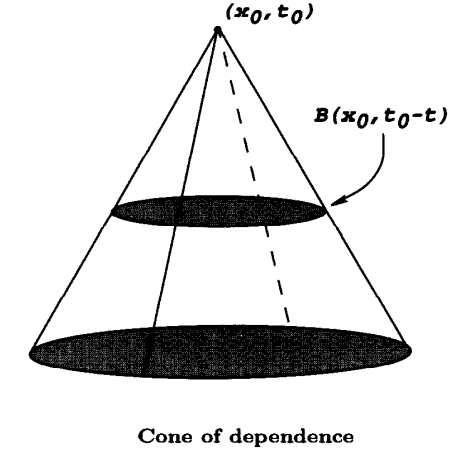
\includegraphics[width=0.5\linewidth]{Graphics/evans_domdependence.png}
		\caption{Depiction of the domain of dependence for a point $(x_0, t_0)$. I.e., the value of $u$ depends only on the points contained inside this cone.}
		\label{fig:dom_dependence}
	\end{figure}
	
	Now we will use the energy method to prove another distinct property of hPDE, the \textit{finite propagation speed}. First, we define what we mean by the \textbf{domain of dependence}. 
	
	\begin{definition}[Domain of Dependence]
		Suppose $u \in C^2(U)$ solves the wave equation 
		\begin{equation*}
			u_{tt} - \Delta u= 0 \qquad (\text{in } \mathbb{R}^n \times (0,\infty)). 
		\end{equation*}
		Fix $x_0 \in \mathbb{R}^n$ and $t_{0} > 0$. Then define the cone 
		\begin{equation}
			C \coloneqq \brac{(x, t) \mid 0 \leq t \leq t_0, |x - x_0| \leq t_0 - t}. 
		\end{equation}
	\end{definition}
	
	In some sense, we have already seen this explicitly in the representation formulas for solutions to the wave equation. However, we will now use energy methods. We have the following theorem. 
	
	\begin{theorem}[Finite Propagation Speed]
		If $u \equiv u_t \equiv 0$ on $B(x_0,t_0)$, then $u \equiv 0$ within the cone $C$. I.e., any disturbance originating outside $B(x_0,t_0)$ has no effect on the solution within $C$, and consequently has finite propagation speed. 
	\end{theorem}
	
	\newpage 
	\subsection{Exercises}
	\begin{prb}{1-1}
		$ $\newline \vspace{-0.25cm}
		\begin{enumerate}[itemsep =-2pt,label = (\alph{*})]
			\item Show the general solution of the PDE $u_{xy} = 0$ is 
			\begin{equation*}
				u(x, y) = F(x) + G(y) 
			\end{equation*}
			for arbitrary functions $F, G$. 
			\item Using the change of variables $\xi = x + t$, $\eta = x - t$, show $u_{tt} - u_{xx} = 0$ if and only if $u_{\xi\eta} = 0$. 
			\item Use (a) and (b) to rederive d'Alembert's formula. 
		\end{enumerate}
	\end{prb}
	\begin{enumerate}[itemsep =-2pt,label = (\alph{*})]
		\item Consider the PDE $u_{xy} =0$. Let $v(x,y) = u_{x}$. Then $v$ satisfies the differential equation $v_{y} = 0$. Thus since $v$ is independent of $y$, one has $u_{x}(x,y) = v(x,y) = f(x)$ for some arbitrary function $f$. But then integrating both sides with respect to $x$, and supposing that $F(x)$ is the antiderivative of $f(x)$, 
		\begin{equation*}
			u(x,y) = F(x) + G(y), 
		\end{equation*}
		where $G$ is some arbitrary function of $y$. 
		\item Define $\xi = x + t$ and $\eta = x -t$ so that $x = (\xi + \eta)/2$ and $t = (\xi - \eta)/2$. Then, 
		\begin{align*}
			\begin{split}
				u_{\xi} &= u_{x}\frac{\partial x}{\partial \xi} + u_{t}\frac{\partial t}{\partial \xi} \\
				&= \frac{1}{2}u_{x} + \frac{1}{2}u_{t}. \\
				u_{\xi\eta} &= \frac{1}{2}\left[u_{xx}\frac{\partial x}{\partial \eta} + u_{xt}\frac{\partial t}{\partial \eta}\right] + \frac{1}{2}\left[u_{tx}\frac{\partial x}{\partial \eta} + u_{tt}\frac{\partial t}{\partial \eta}\right] \\
				&= \frac{1}{2}[u_{xx} -u_{xt}] + \frac{1}{2}[u_{tx} - u_{tt}] =  \frac{1}{2}[u_{tt} - u_{xx}], 
			\end{split}
		\end{align*}
		where we used the fact that $u_{xt} = u_{tx}$. Thus, the proof concludes. 
		\item Consider the initial value problem, 
		\begin{equation*}
			\left\{
			\begin{alignedat}{3}
				&u_{tt} -u_{xx} &= 0 \qquad &(\text{in $\mathbb{R} \times (0,\infty)$}) \\
				&u = g, u_{t} &= h \qquad &(\text{on $\mathbb{R} \times \{t = 0\}$}).
			\end{alignedat}
			\right.
		\end{equation*}
		Define the change of variables $\xi = x + t$ and $\eta = x - t$ as above. By (b), $u_{tt} - u_{xx} = 0$ if and only if $u_{\xi\eta} =0$. By (a), it follows that $u$ must be of the form, 
		\begin{equation*}
			u(\xi, \eta) = F(\xi) + G(\eta). 
		\end{equation*}
		Thus, $u(x,t) = F(x + t) + G(x - t)$. Now we must match the initial conditions. At $t = 0$, 
		\begin{align*}
			\begin{split}
				u(x, 0) &= F(x) + G(x) = g(x). \\
				u_{t}(x, 0) &= F'(x) - G'(x) = h(x). 
			\end{split}
		\end{align*}
		Differentiating the first equation, one first obtains the system 
		\begin{equation*}
			\left\{
			\begin{alignedat}{2}
				&F'(x) + G'(x) &= g'(x) \\
				&F'(x) - G'(x) &= h(x). 
			\end{alignedat}
			\right. 
		\end{equation*} 
		Thus, we get 
		\begin{equation*}
			F'(x) = \frac{1}{2}(g'(x) +h(x)) \implies F(x + t) = \frac{1}{2}[g(x+ t) - g(0)] + \frac{1}{2}\int_{0}^{x + t}h(y)\;dy + F(0). 
		\end{equation*}
		Likewise, we get 
		\begin{equation*}
			G(x-t) = \frac{1}{2}[g(x - t) - g(0)] -\int_{0}^{x - t}h(y)\;dy + G(0). 
		\end{equation*}
		Adding the two equations, and using the fact that $F(0) + G(0) = g(0)$, we conclude that 
		\begin{equation*}
			u(x,t) = \frac{1}{2}[g(x - t) + g(x + t)] + \frac{1}{2}\int_{x - t}^{x + t}h(y)\;dy, 
		\end{equation*}
		which is precisely d'Alembert's formula. 
	\end{enumerate}
	
	\begin{prb}{1-2}
		Assume $\mathbf{E} = (E^{1}, E^{2}, E^{3})$ and $\mathbf{B} = (B^{1}, B^{2}, B^{3})$ solve Maxwell's equations. Show 
		\begin{equation*}
			u_{tt} - \Delta u= 0
		\end{equation*}
		where $u = E^{i}$ or $B^{i}$ ($i = 1, 2, 3$). 
	\end{prb}
	Recall that Maxwell's equations are given by the following system, 
	\begin{equation*}
		\left\{
		\begin{alignedat}{1}
			&\mathbf{E}_{t} = \nabla \times \mathbf{B} \\
			&\mathbf{B}_{t} = -\nabla \times \mathbf{E} \\
			&\mathbf{\nabla} \cdot \mathbf{B}= \nabla \cdot \mathbf{E} =0. 
		\end{alignedat}
		\right.
	\end{equation*}
	Assume $\mathbf{E} = (E^{1}, E^{2}, E^{3})$ and $\mathbf{B} = (B^{1}, B^{2}, B^{3})$ solve Maxwell's equations. Then differentiating the first equation and using the fact that time derivatives commute with spatial derivatives, one obtains 
	\begin{equation*}
		\mathbf{E}_{tt} = \nabla \times \mathbf{B}_{t} = -\nabla \times (\nabla \times E) = -\nabla (\nabla \cdot \mathbf{E}) + \Delta \mathbf{E} = \Delta \mathbf{E}, 
	\end{equation*}
	where the final equality follows from the fact that $\nabla \cdot \mathbf{E} = 0$. Thus, we have 
	\begin{equation*}
		\mathbf{E}_{tt} - \Delta \mathbf{E} = 0 \iff (E^{1}_{tt} - \Delta E^{1}, \ldots, E^{3}_{tt} - \Delta E^{3}) = \mathbf{0}. 
	\end{equation*}
	Hence, each $E^{i}$ satisfies the wave equation. Now differentiate the second equation. We get 
	\begin{equation*}
		\mathbf{B}_{tt} =-\nabla \times \mathbf{E}_{t} = -\nabla \times (\nabla \times \mathbf{B}) = -\nabla (\nabla \cdot \mathbf{B}) + \Delta \mathbf{B} = \Delta \mathbf{B}. 
	\end{equation*}
	Thus we have, 
	\begin{equation*}
		\mathbf{B}_{tt} - \Delta \mathbf{B} = 0 \iff (B^{1}_{tt} - \Delta B^{1}, \ldots, B^{3}_{tt} - \Delta B^{3}) = \mathbf{0}. 
	\end{equation*}
	Therefore, each $B^{i}$ satisfies the wave equation. 
	
	\begin{prb}{1-3}
		(Equipartition of Energy). Let $u \in C^{2}(\mathbb{R} \times [0,\infty))$ solve the initial-value problem for the wave equation in one-dimension: 
		\begin{equation*}
			\left\{
			\begin{alignedat}{3}
				&u_{tt} - u_{xx} &=0 \qquad &(\text{in } \mathbb{R} \times (0,\infty)) \\
				&u=g, u_t &= h \qquad &(\text{on } \mathbb{R} \times \{t = 0\}).
			\end{alignedat}
			\right. 
		\end{equation*} 
		Suppose $g,h$ have compact support. The \textit{kinetic energy} is $k(t) \coloneqq \frac{1}{2}\int_{-\infty}^{\infty}u_t^2(x,t)\;dx$ and the \textit{potential energy} is $p(t) \coloneqq \frac{1}{2}\int_{-\infty}^{\infty}u_x^2(x,t)\;dx$. Prove \vspace{-0.25cm}
		\begin{enumerate}[itemsep =-2pt,label =(\roman{*})]
			\item $k(t) + p(t)$ is constant in $t$, 
			\item $k(t) = p(t)$ for all large enough times $t$. 
		\end{enumerate}
	\end{prb}
	\begin{enumerate}[itemsep =-2pt,label = (\roman{*})]
		\item Let us define the kinetic and potential energy, $k(t)$ and $p(t)$ as given above. We wish to show that the total energy 
		\begin{equation*}
			e(t) = k(t) + p(t) = \frac{1}{2}\int_{-\infty}^{\infty}u_t^2 + u_x^2\;dx
		\end{equation*}
		is conserved, where $u$ is given by d'Alembert's formula, 
		\begin{equation*}
			u(x, t) = \frac{1}{2}[g(x + t) + g(x - t)] + \frac{1}{2}\int_{x - t}^{x + t}h(y)\;dy. 
		\end{equation*}
		so that 
		\begin{align*}
			\begin{split}
				u_t(x,t) &= \frac{1}{2}[g'(x + t) - g'(x - t) + h(x + t) + h(x - t)]. \\
				u_x(x, t) &= \frac{1}{2}[g'(x + t) + g'(x - t) + h(x + t) - h(x - t)]. 
			\end{split}
		\end{align*}
		Let $T > 0$, and let $K \subset \mathbb{R}$ be a compact set large enough so that $\operatorname{supp}{g}, \operatorname{supp}{h}$ are both contained in $K$. Then it follows that $u_t^2$ and $u_x^2$ are both supported in $K_{T} \coloneqq K + [-T,T]$ for all $0 \leq t \leq T$. Since $u_t^2$ and $u_x^2$ are continuous on $\mathbb{R}$ (and thus on $K_T$) for all $0 \leq t \leq T$, by the extreme value theorem, there exist finite constants $M$ and $N$ so that for all $x \in K$ and $0 \leq t \leq T$, $|u_t|^2 \leq M\chi_{K_T}$ and $|u_x^2| \leq N\chi_{K_T}$, where both dominating functions are integrable since $K_{T}$ is compact. Thus using the Dominated Convergence Theorem, taking the derivative of $e(t)$ gives us, 
		\begin{align*}
			\begin{split}
				\dot{e}(t) &= \frac{1}{2}\frac{\partial}{\partial t}\int_{-\infty}^{\infty}u_t^2 + u_x^2\;dx = \frac{1}{2}\frac{\partial}{\partial t}\int_{K_T}u_t^2 + u_x^2\;dx \\
				&= \frac{1}{2}\int_{K_T}\partial_t(u_t^2 + u_x^2)\;dx \\
				&= \int_{K_T}u_tu_{tt} + u_x \cdot \partial_x u_t\;dx \\
				&= \int_{K_T}u_t(u_{tt} - u_{xx})\;dx \qquad (\text{by integration by parts}) \\
				&= 0, 
			\end{split}
		\end{align*}	
		where there is no boundary term since $u_x, u_t$ are supported inside $K_T$. So we have shown that $\dot{e}(t) = 0$ for all $0 \leq t \leq T$. Since $T > 0$ was chosen arbitrarily, it follows that $\dot{e}(t)\equiv 0$. Therefore, the total energy is constant in $t$. 
		\item What we wish is that in the limit $t \to \infty$, 
		\begin{equation*}
			\abs{\int_{\mathbb{R}}u_t^2 - u_x^2\;dx} \to 0. 
		\end{equation*}
		First, we compute 
		\begin{equation*}
			u_t^2 - u_x^2 = h(x + t)h(x - t) - h(x + t)g'(x - t) + h(x - t)g'(x + t) - g'(x - t)g'(x + t). 
		\end{equation*}
		Then 
		\begin{align*}
			\begin{split}
				\abs{\int_{\mathbb{R}}u_t^2 - u_x^2\;dx} &\leq \int_{-\infty}^{\infty}|h(y)h(y - 2t)|\;dy + \int_{-\infty}^{\infty}|h(y)g'(y - 2t)|\;dy \\
				&\quad+ \int_{-\infty}^{\infty}|h(y - 2t)g'(y)|\;dy + \int_{-\infty}^{\infty}|g'(y - 2t)g'(y)|\;dy.
			\end{split}
		\end{align*}
		Let $K \subset \mathbb{R}$ be a compact set large enough that contains the support of both $g$ and $h$. Then we may write, 
		\begin{align*}
			\begin{split}
				\abs{\int_{\mathbb{R}}u_t^2 - u_x^2\;dx} &\leq \int_{K}|h(y)h(y - 2t)|\;dy + \int_{K}|h(y)g'(y - 2t)|\;dy \\
				&\quad+ \int_{K}|h(y - 2t)g'(y)|\;dy + \int_{K}|g'(y - 2t)g'(y)|\;dy.
			\end{split}
		\end{align*}
		We will only show that the first term on the right vanishes since the work for the remaining terms is identical. Since $h(u) \to 0$ as $|u| \to \infty$ (by compact support of $h$), we know that pointwise $|h(y)h(y - 2t)| \to 0$ as $t \to \infty$. Next since $h$ is continuous, there exists some finite $M > 0$ so that $|h(y)|, |h(y - 2t)| \leq M$ for all $y \in K$. Thus, $|h(y)h(y-2t)| \leq M^2\chi_{K} \in L^1(\mathbb{R})$ since $K$ is compact. Hence, by the Dominated Convergence Theorem, one has that the first term vanishes as $t \to \infty$. As we stated before, the remaining three terms also vanish as $t \to \infty$. Thus, we conclude that as $t \to \infty$,
		\begin{equation*}
			\abs{\int_{\mathbb{R}}u_t^2 - u_x^2\;dx} \to 0. 
		\end{equation*}
	\end{enumerate}
	
	\begin{prb}{12-6}
		Let $u$ solve 
		\begin{equation*}
			\left\{
			\begin{alignedat}{3}
				&u_{tt} - \Delta u &=0 &\qquad \text{in $\mathbb{R}^3 \times (0,\infty)$} \\
				&u = g, u_t &= h &\qquad \text{on $\mathbb{R}^3 \times \{t = 0\}$},
			\end{alignedat}
			\right.
		\end{equation*}
		where $g, h$ are smooth and have compact support. Show there exists a constant $C$ such that 
		\begin{equation*}
			|u(x,t)| \leq C/t \qquad (x \in \mathbb{R}^3, t > 0). 
		\end{equation*}
	\end{prb}
	Let $u$ be the solution to the initial value problem given above. We recall that $u$ is given by Kirchoff's formula, 
	\begin{equation*}
		u(x,t) = \dashint_{\partial B(x,t)}th(y) + g(y) + Dg(y) \cdot (y - x)\;dS(y) \qquad (x \in \mathbb{R}^3, t > 0)
	\end{equation*}
	Let $R > 0$ be a fixed positive constant so that the support of $g$ and $h$ are both contained inside the ball $B(0,R)$. We can rewrite, 
	\begin{align*}
		\begin{split}
			|u(x,t)| &\leq \frac{1}{4\pi t^2}\left[\underbrace{\int_{\partial B(x,t)}t|h(y)|\;dS(y)}_{(a)} + \underbrace{\int_{\partial B(x,t)}|g(y)|\;dS(y)}_{(b)} + \underbrace{\int_{\partial B(x,t)}|Dg(y)\|y-x|\;dS(y)}_{(c)}\right]. 
		\end{split}
	\end{align*}
	We will try bounding each term independently. 
	\begin{enumerate}[itemsep =-2pt,label = (\alph{*})]
		\item Let us denote $\Sigma_t = \partial B(x,t) \cap B(0,R)$. Then it follows that 
		\begin{equation*}
			\int_{\partial B(x,t)}t|h(y)|\;dS(y) = t\int_{\Sigma_t}|h(y)|\;dS(y) \leq tM\cdot 4\pi R^2, 
		\end{equation*}
		where $M > 0$ is a constant so that $|h|\leq M$, and we used the fact that the surface area of $\partial B(x,t) \cap B(0,R)$ cannot exceed the surface area of $4\pi R^2$.\footnote{\href{https://math.stackexchange.com/questions/1302682/2d-wave-equation-decay-estimate}{https://math.stackexchange.com/questions/1302682/2d-wave-equation-decay-estimate}} 
		\item Now let $N > 0$ so that $|g|\leq N$. Then repeating the work from above shows that 
		\begin{equation*}
			\int_{\partial B(x,t)}|g(y)|\;dS(y) \leq N \cdot 4\pi R^2.
		\end{equation*}
		\item Now we note that for all $y \in \partial B(x,t)$, $|y - x| = t$. So taking $L > 0$ so that $|Dg| \leq L$, and repeating the work from (a), one has that 
		\begin{equation*}
			\int_{\partial B(x,t)}|Dg(y)\|y - x|\;dS(y) = t L \cdot 4\pi R^2. 
		\end{equation*}
	\end{enumerate}
	Combining all of the pieces together, we find that 
	\begin{align*}
		\begin{split}
			|u(x,t)| &\leq \frac{1}{4\pi t^2} \cdot \left[4\pi R^2(M + L)t + 4\pi R^2N\right] \\
			&\leq \frac{1}{t^2} \cdot C'(1 + t) \leq \frac{C}{t}
		\end{split}
	\end{align*}
	
	\begin{prb}{12-5}
		Let $u$ solve 
		\begin{equation*}
			\left\{
			\begin{alignedat}{3}
				&u_{tt} - \Delta u &=0 &\qquad \text{in $\mathbb{R}^3 \times (0,\infty)$} \\
				&u = g, u_t &= h &\qquad \text{on $\mathbb{R}^3 \times \{t = 0\}$},
			\end{alignedat}
			\right.
		\end{equation*}
		where $g, h$ have compact support. Show that    
		\begin{equation*}
			|u(x,t)| \leq C/t^{\frac{1}{2}} \qquad (x \in \mathbb{R}^2, t > 0)
		\end{equation*}
		for some constant $C$. 
	\end{prb}
	Let $u$ be a solution to the initial value problem for the wave equation on $\mathbb{R}^2$, where the initial data are compactly supported. We recall that $u$ is given by Poisson's Formula, 
	\begin{equation*}
		u(x, t)= \frac{1}{2}\dashint_{B(x,t)}\frac{tg(y) + t^2h(y) + tDg(y) \cdot (y - x)}{(t^2 - |y - x|^2)^{1/2}}\;dy \qquad (x \in \mathbb{R}^2, t > 0).
	\end{equation*}
	Let $R > 0$ be large enough so that the ball $B(0,R)$ contains the support of both $g$ and $h$. We begin by writing, 
	\begin{equation*}
		u(x,t) = \frac{1}{2\pi t^{2}}\left[\underbrace{\int_{B(x,t)}\frac{tg(y)}{(t^2 - |y - x|^2)^{1/2}}\;dy}_{(a)} + \underbrace{\int_{B(x,t)}\frac{t^2h(y)}{(t^2 - |y - x|^2)^{1/2}}\;dy}_{(b)} + \underbrace{\int_{B(x,t)}\frac{tDg(y) \cdot (y -x)}{(t^2 - |y - x|^2)^{1/2}}\;dy}_{(c)} \right]. 
	\end{equation*}
	We will look at each of the above terms independently. 
	\begin{enumerate}[itemsep =-2pt,label = (\alph{*})]
		\item Since the support of $g$ is contained in $B(0,R)$, we can write 
		\begin{align*}
			\begin{split}
				\int_{B(x,t)}\frac{t|g(y)|}{(t^2 - |y - x|^2)^{1/2}}\;dy &= \int_{B(x, t) \cap B(0,R)}\frac{t|g(y)|}{(t^2 - |y - x|^2)^{1/2}}\;dy  \\
				&\leq \int_{B(x,t) \cap B(0,R)}\frac{tM}{(t + |y - x|)^{1/2}(t - |y - x|)^{1/2}}\;dy. 
			\end{split}
		\end{align*}
		where $M > 0$ is chosen such that $|g(y)| \leq M$ for all $y \in B(0,R)$. Now let us switch to polar coordinates: 
		\begin{align*}
			\begin{split}
				
			\end{split}
		\end{align*}
	\end{enumerate}
	
	\begin{prb}{1-5}
		(Stokes' Rule) Assume $u$ solves the initial-value problem 
		\begin{equation*}
			\left\{
			\begin{alignedat}{3}
				&u_{tt} - \Delta u &= 0 &\qquad \text{in $\mathbb{R}^n \times (0,\infty)$} \\
				&u =0, u_t &=h &\qquad \text{on $\mathbb{R}^n \times \{t = 0\}$}.
			\end{alignedat}
			\right.
		\end{equation*}
		Show that $v \coloneqq u_t$ solves 
		\begin{equation*}
			\left\{
			\begin{alignedat}{3}
				&v_{tt} - \Delta v &= 0 &\qquad \text{in $\mathbb{R}^n \times (0,\infty)$} \\
				&v =h, v_t &= 0 &\qquad \text{on $\mathbb{R}^n \times \{t = 0\}$}.
			\end{alignedat}
			\right.
		\end{equation*}
		This is \textit{Stokes' rule}. 
	\end{prb}
	Assume $u$ solves the given initial value problem, and set $v \coloneqq u_t$. The boundary value conditions for $v$ are immediately clear by the initial value problem for $u$. Thus, it suffices to show that $\Box v = 0$. Observe the following: 
	\begin{align*}
		\begin{split}
			v_{tt} &= u_{ttt}. \\
			\Delta v &= \Delta (u_{t}) = \partial_{t}(\Delta u) = \partial_t (u_{tt}) = u_{ttt}. 
		\end{split}
	\end{align*}
	This implies that $v_{tt} - \Delta v = u_{ttt} - u_{ttt} =0$. Thus the proof concludes. 
	
	\newpage 
	\section{General Analytic Techniques}
	In this section, we will revisit the linear wave equation. This time, however, we will be doing so from the lens of Fourier/harmonic analysis, and functional analysis. We will begin with a review of essential Fourier Theory. 
	
	\subsection{Fourier Theory and the Linear Wave Equation}
	\subsubsection{The Fourier Transform}
	In this section, we will be using the following function spaces extensively, 
	\begin{enumerate}[itemsep =-2pt,label = (\arabic{*})]
		\item Let $U \subseteq \mathbb{R}^{n}$ be an open subset. Then we define the space $C^{\infty}(U)$ to be the space of all smooth functions. We define $C_{c}^{\infty}(U)$ to be the space of all smooth functions in $U$ whose support is compact. 
		\item We define the \textbf{Schwartz space} on $\mathbb{R}^{n}$ to be the space, 
		\begin{equation}
			\mathcal{S}(\mathbb{R}^n) \coloneqq \brac*{f \in C^{\infty}(\mathbb{R}^n): \sup_x|x^\alpha\partial^\beta_xf| \leq C_{\alpha,\beta} \text{ for all multiindices $\alpha,\beta$}}. 
		\end{equation}
		I.e., the Schwartz space is comprised of smooth function that ``decay faster than polynomials.'' 
		\item The function space, $L^p(\mathbb{R}^n)$, $1 \leq p < \infty$, is the completion of $\mathcal{S}(\mathbb{R}^n)$ under the $L^p$-norm. 
	\end{enumerate}
	Given these spaces, we define the \textbf{Fourier transform} of an integrable function as follows. 
	\begin{definition}[Fourier Transform of an Integrable Function]
		Let $f \in L^1(\mathbb{R}^n)$. Then its \textbf{Fourier transform} is the function, 
		\begin{equation}
			\hat{f}(\xi) \coloneqq \int_{\mathbb{R}^n}f(x)e^{-2\pi i x \cdot \xi}\;dx. 
		\end{equation}
		Note that since $f \in L^1$, so is its Fourier transform $\hat{f}$. 
	\end{definition}
	
	Conversely, given a function $\hat{f}(\xi) \in L^1(\mathbb{R}^n)$, we can define its \textbf{inverse Fourier transform} as follows. 
	\begin{definition}[Inverse Fourier Transform]
		Given $g \in L^{1}(\mathbb{R}^n)$, its inverse Fourier transform is the function 
		\begin{equation*}
			\check{g}(x) = \int_{\mathbb{R}^n}g(x)e^{2\pi i x \dot \xi}\;d\xi. 
		\end{equation*}
	\end{definition}
	This prompts the following theorem (see Appendix for the proof). 
	\begin{theorem}[Basic Properties of the Fourier Transform]
		$ $\newline \vspace{-0.65cm}
		\begin{enumerate}[itemsep =-2pt,label = (\arabic{*})]
			\item (Fourier Inversion Formula) For $f$ such that $f, \hat{f} \in L^1(\mathbb{R}^n)$, we have $(\hat{f})^{\check{}} = f$ almost everywhere. 
			\item The Fourier transform maps the Schwartz space onto itself. 
			\item (Plancherel's Theorem) Let $f \in L^1 \cap L^2(\mathbb{R}^n)$. Then 
			\begin{equation}
				\|\hat{f}\|_{L^2(\mathbb{R}^n)} = \norm{f}_{L^2(\mathbb{R}^n)}. 
			\end{equation}
			As a consequence, the Fourier transform extends (by density) to an isometric isomorphism $L^2(\mathbb{R}^n) \to L^2(\mathbb{R}^n)$. 
			\item For any $\phi \in C^\infty(\mathbb{R}^n)$, 
			\begin{equation}
				\mathcal{F}(\partial_i\phi)(\xi) = 2\pi i \xi_i\hat{\phi}(\xi). 
			\end{equation}
			I.e., the Fourier transformation turns differentiation in a variable to multiplication in the conjugate variable. 
		\end{enumerate}
		\label{thm:prop_four_transform}
	\end{theorem}
	
	\subsubsection{Solution to the Wave Equation in Fourier Space}
	We will now explicitly construct a solution to the wave equation by using Fourier transforms. Consider the wave equation, $\phi_{tt} - \Delta \phi = 0$, where we assume at least that $\phi \in L^1(\mathbb{R}^n)$. Then taking the Fourier transform of both sides, one has 
	\begin{equation*}
		-\partial_{t}^2\hat{\phi}(\xi) - 4\pi |\xi|^{2}\hat{\phi}(\xi) = 0, 
	\end{equation*}
	which is an ordinary differential equation (ODE). Solving this ODE, one obtains the general solution, 
	\begin{equation*}
		\hat{\phi}(t, \xi) = A(\xi)\sin(2\pi t|\xi|) + B(\xi)\cos(2\pi t|\xi|). 
	\end{equation*}
	Suppose we are also given the initial conditions, $(\phi_{0}, \phi_1) \in C_{c}^{\infty}(\mathbb{R}^n) \times C_{c}^{\infty}(\mathbb{R}^n) \subset \mathcal{S}(\mathbb{R}^n) \times \mathcal{S}(\mathbb{R}^n)$. Then matching initial conditions gives us, 
	\begin{equation}
		\hat{\phi}(t, \xi) = \frac{\hat{\phi}_{1}(\xi)}{2\pi |\xi|}\sin(2\pi t |\xi|) + \hat{\phi}_{0}(\xi)\cos(2\pi t|\xi|). 
	\end{equation}
	Thus under these assumptions, we have shown the existence of a solution to the wave equation (again, this is not a new result as we have already derived explicit representation formulas). Likewise, we have the following proof that the energy is conserved (cf. Problem 3 in the Exercises section above). 
	
	\begin{prop}[Conservation of Energy]
		For $(\phi_0, \phi_1) \in C_c^{\infty}(\mathbb{R}^n) \times C_c^{\infty}(\mathbb{R}^n)$ and $\phi$ the unique solution to the initial value problem for the linear wave equation, one has that the energy, 
		\begin{equation*}
			e(t) \coloneqq \frac{1}{2}\int_{\mathbb{R}^n}\phi_t^2 + \Delta\phi\;dx
		\end{equation*}
		is independent of $t$. 
	\end{prop}
	\begin{proof}
		Since $C_{c}^{\infty}(\mathbb{R}^n) \subset L^2(\mathbb{R}^n)$, one has by Plancherel's theorem that 
		\begin{equation*}
			e(t) = \frac{1}{2}\int_{\mathbb{R}^n}\hat{\phi}_t^2 + \sum_1^n(2\pi \xi_i\hat{\phi})^2\;d\xi. 
		\end{equation*}
		We will show that the integrand is independent of time. First, we compute the following, 
		\begin{align*}
			\begin{split}
				|\hat{\phi}_t|^2 &= (\hat{\phi}_1\cos(2\pi t|\xi|) - \hat{\phi}_0 \cdot 2\pi |\xi|\sin(2\pi t|\xi|))^2. \\
				\sum_1^n(2\pi \xi_i\hat{\phi})^2 &= |\hat{\phi}_1(\xi)|^2\sin^2(2\pi|\xi|t) \\
				&\qquad + 4\pi^2|\xi|^2|\hat{\phi}_0(\xi)|^2\cos^2(2\pi |\xi|t) + 4\pi |\xi|\hat{\phi}_0(\xi)\hat{\phi}_1(\xi)\sin(2\pi t |\xi|)\cos(2\pi t|\xi|). \\
				|\hat{\phi}_t|^2 + \sum_1^n(2\pi \xi_i\hat{\phi})^2 &= |\hat{\phi}_1(\xi)|^2 + 4\pi^2|\xi|^2|\hat{\phi}_0(\xi)|^2, 
			\end{split}
		\end{align*}
		which is independent of time. Thus, $e(t)$ is independent of time. Note that this proof is much shorter than the proof given in Problem 3. 
	\end{proof}
	
	The following propositions, however, are much more foundational. For $n \geq 2$, the solutions to the wave equation on $\mathbb{R}^n$ \textit{decay} as $t \to \infty$ (see Figure \ref{fig:dispersionn2}). The following propositions give simple decay rates for these solutions. 
	
	\begin{prop}[Decay Rate I]
		Fix any $R > 0$. For $(\phi_0, \phi_1) \in C_c^\infty(\mathbb{R}^n) \times C_c^\infty(\mathbb{R}^n)$, and $\phi$ the unique solution to the initial value problem for the linear wave equation ($n \geq 2$), there exists $C = C(\phi_0,\phi_1,R) > 0$ such that 
		\begin{equation}
			\sup_{\{|x| \leq R\}}|\phi(t,x)| \leq \frac{C}{(1 + t)^{n-1}} \qquad \forall t \geq 0. 
		\end{equation}
	\end{prop}
	
	\begin{figure}[t!]
		\centering
		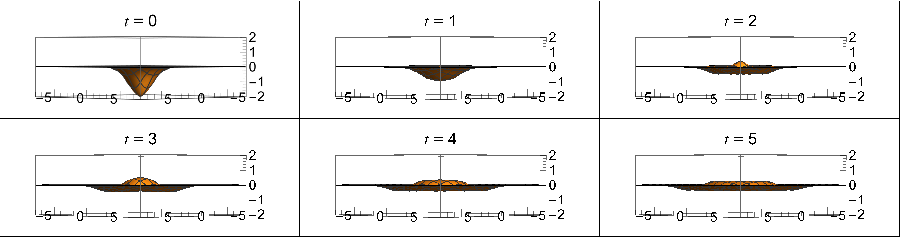
\includegraphics[width=\linewidth]{Graphics/dispersion_n2.pdf}
		\caption{Dispersion in the solution for the wave equation ($n = 2$).}
		\label{fig:dispersionn2}
	\end{figure}
	\begin{proof}
		Before proceeding with the proof, we rewrite the solution $\hat{\phi}$ as follows: 
		\begin{equation}
			\hat{\phi}(\xi,t) = e^{2\pi i |t|\xi}\left(\frac{\hat{\phi}_0(\xi)}{2} + \frac{\hat{\phi}_1(\xi)}{2\pi i |\xi|}\right) + e^{-2\pi i t|\xi|}\left(\frac{\hat{\phi}_0(\xi)}{2} - \frac{\hat{\phi}_1(\xi)}{2\pi i |\xi|}\right). 
		\end{equation}
		In this proof, we only consider the case $n = 3$, and the integral 
		\begin{equation*}
			I = \int_{\mathbb{R}^3}e^{2\pi i (t |\xi| + x \cdot \xi)} \frac{\hat{\phi}_1(\xi)}{2\pi i |\xi|}\;d\xi. 
		\end{equation*}
		Furthermore, we will only consider the case $t \geq 1$. We begin by writing $\xi$ using the polar coordinates $(|\xi|, \xi_\theta, \xi_\varphi)$, defined as follows:
		\begin{equation*}
			|\xi|^2 = \xi_1^2 + \dotsm + \xi_3^2, \quad \xi_3 = |\xi|\cos{\xi_\theta}, \quad \xi_3 = |\xi|\sin{\xi_\theta}\cos{\xi_\varphi}. 
		\end{equation*}
		In this coordinate system, the volume form is $d\xi = |\xi|^2\sin{\xi_\theta}\;d|\xi|d\xi_\theta d\xi_\varphi$. Quickly note that for any nonnegative integer $N$, 
		\begin{equation*}
			\left(\frac{1}{2\pi it}\frac{\partial}{\partial |\xi|}\right)^Ne^{2\pi i t|\xi|} = e^{2\pi i t|\xi|}. 
		\end{equation*}
		Now using integration by parts, 
		\begin{align*}
			\begin{split}
				I &= \int_0^{2\pi}\int_0^\pi\int_0^\infty e^{2\pi i t|\xi|} e^{2\pi i (x \cdot \xi)} \frac{\hat{\phi}_1(\xi)}{2\pi i}|\xi|\sin(\xi_\theta)\;d|\xi|d\xi_\theta d\xi_\varphi \\
				&= \left[ \frac{1}{(2\pi i)^2 t}\int_0^{\pi}\int_0^{2\pi}e^{2\pi i t |\xi|}e^{2\pi i (x \cdot \xi)}\hat{\phi}_1(\xi) |\xi| \sin(\xi_\theta)\;d\xi_\varphi d\xi_\theta \right]^{R \to \infty}_{|\xi| = 0} \\
				&\qquad - \int_0^{2\pi}\int_0^\pi\int_0^\infty \frac{1}{2\pi i t} e^{2\pi i t|\xi|} \frac{\partial}{\partial |\xi|}\left(e^{2\pi i x \cdot \xi}\frac{\hat{\phi}_1(\xi)}{2\pi i}|\xi|\right)\sin(\xi_\theta)\;d|\xi| d\xi_\theta d\xi_\varphi
			\end{split}
		\end{align*}
		We claim that the first term is identically zero. To prove this, we first note that 
		\begin{equation*}
			\lim_{|\xi|\to \infty}\abs{^{2\pi i t |\xi|}e^{2\pi i (x \cdot \xi)}\hat{\phi}_1(\xi) |\xi| \sin(\xi_\theta)} = \lim_{|\xi| \to \infty}|\hat{\phi}_1(\xi)||\xi| = 0, 
		\end{equation*}
		since $\hat{\phi}_1(\xi) \in \mathcal{S}(\mathbb{R}^3)$. On the other hand, the integrand vanishes identically at $|\xi| = 0$. Now, we see that one application of integration by parts gave us a power of $t$. To get another power of $t$, we will use integration by parts on the second term. This time, after dealing with a boundary term at $|\xi| = 0$, we get 
		\begin{equation*}
			I = -\int_{\mathbb{R}^3}e^{2\pi i t|\xi|}\frac{1}{8\pi^3it^2}\left(\dotsm\right)\sin(\xi_\theta)\;d|\xi|d\xi_\theta d\theta_\varphi + \frac{1}{2\pi^2 i t^2}\hat{\phi}_1(\xi = 0). 
		\end{equation*}
		The boundary term does not allow us to use integration by parts again. Thus bounding each of the term and using the fact that $\hat{\phi}_1 \in \mathcal{S}$, one obtains 
		\begin{equation*}
			|I| \leq \frac{C(1 + R^2)}{t^2}. 
		\end{equation*}
		Note that this decay bound is not uniform for all $x \in \mathbb{R}^n$. 
	\end{proof}
	
	However, we can get a \textit{weaker uniform} decay rate. 
	
	\begin{theorem}[Uniform Decay Rate]
		For $(\phi_0, \phi_1) \in C_c^{\infty}(\mathbb{R}^n) \times C_c^{\infty}(\mathbb{R}^n)$, and $\phi$ the unique solution to the homogeneous initial value problem, there exists $C = C(\phi_0, \phi_1) > 0$ so that
		\begin{equation*}
			\sup_{x \in \mathbb{R}^n}|\phi(t,x)| \leq \frac{C}{(1 + t)^{\frac{n-1}{2}}}
		\end{equation*}
		for $t\geq 0$. 
	\end{theorem}
	
	\subsection{Distribution Theory and the Linear Wave Equation}
	\subsubsection{A Short Introduction to Distribution Theory}
	In this section, we will quickly introduce a few key ideas of distribution theory, and then use these ideas to obtain the \textbf{fundamental solution} to the equation $\Box E = \delta_0$. We will use this fundamental solution to construct the solution to the wave equation in physical space. We begin with a couple of definitions. 
	
	\begin{definition}[Distributions]
		Let $U \subseteq \mathbb{R}^n$ be an open subset. \vspace{-0.25cm}
		\begin{enumerate}[itemsep =-2pt,label = (\arabic{*})]
			\item A \textbf{distribution} in an open set $U \subseteq \mathbb{R}^n$ is a linear map $u: C_c^\infty(U) \to \mathbb{R}$ such that for \textit{every} compact set $K \subseteq U$, there exists $C > 0$ and $k \in \mathbb{N} \cup \{0\}$ such that 
			\begin{equation*}
				|u(\varphi)| \leq C \sum_{|\alpha|\leq k}\sup_{x \in K}|\partial^\alpha \varphi(x)|, 
			\end{equation*}
			for all $\varphi \in C_c^\infty(K)$. We will denote $\braket{u,\varphi} \coloneqq u(\varphi)$, and we will denote the space of all distributions on $U$ by $\mathcal{D}'(U)$. 
			\item Let $V \subseteq U \subseteq \mathbb{R}^n$ and $u \in \mathcal{D}'(U)$. We define the \textbf{restriction of $u$ to $V$}, denoted $u_V$ by $\braket{u_V, \varphi} \coloneqq \braket{u,\varphi}$ for all $\varphi \in C_c^\infty(V)$. 
			\item Let $U \subseteq \mathbb{R}^n$ be open and $u \in \mathcal{D}'(U)$. The \textbf{support of $u$}, denoted $\operatorname{supp}{u}$, is defined to be the set of all points in $U$ having no open neighborhood to which the restriction of $u$ is 0. 
			\item Let $U \subseteq \mathbb{R}^n$ be open and $u \in \mathcal{D}'(U)$. The \textbf{distributional derivative} of $u$, denoted $\partial^\alpha u$ is defined to be the distribution such that $\braket{\partial^\alpha u,\varphi} = (-1)^{|\alpha|}\braket{u,\partial^\alpha \varphi}$ for all test functions $\varphi$ on $U$. 
		\end{enumerate}
	\end{definition}
	
	We have the following essential facts about distributions (see, e.g., Folland \textit{Real Analysis} for proofs). 
	\begin{prop}[Basic Properties of Distributions]
		Let $U \subseteq \mathbb{R}^n$ be an open subset, and $u \in \mathcal{D}'(U)$. \vspace{-0.25cm}
		\begin{enumerate}[itemsep =-2pt,label = (\arabic{*})]
			\item (Approximation by $C^\infty$ Functions) If $U \subseteq \mathbb{R}^n$ is open and $u \in \mathcal{D}'(U)$, then there exists a sequence $u_j \in C_c^\infty(U)$ such that $u_j \to u$ in $\mathcal{D}'(u)$; i.e., for every $\varphi \in C_c^\infty(U)$, $\int_U u_j\varphi \to \braket{u,\varphi}$. 
			\item (Composition with Smooth Maps) Let $U \subseteq \mathbb{R}^n$ and let $f: U \to \mathbb{R}$ be a smooth map such that $df \neq 0$. Then there exists a continuous map $f^\ast: \mathcal{D}'(\mathbb{R}) \to \mathcal{D}'(U)$ such that $f^\ast u = u \circ f$ whenever $u$ is a continuous function. Given a distribution $u \in \mathcal{D}'(\mathbb{R})$, this can be defined as the limit of $u_j \circ f$, where $u_j \to u$ and $u_j \in C_c^\infty(\mathbb{R})$. 
			\item (Chain Rule) Let $u \in \mathcal{D}'(\mathbb{R})$, $U \subseteq \mathbb{R}^n$, and $f: U \to \mathbb{R}$ be a smooth map such that $df \neq 0$. Then the distributional derivative satisfies the chain rule $\partial(u \circ f) = (\partial f)(u' \circ f)$. 
		\end{enumerate}
	\end{prop}
	Now we need a notion of the convolution of distributions. We make the following definition, 
	\begin{definition}[Convolution of Distributions with Test Functions]
		Let $u \in \mathcal{D}'(\mathbb{R}^n)$ and $\varphi \in C_c^\infty(\mathbb{R}^n)$. Define $(u \ast \varphi)(x) \coloneqq \braket{u, \varphi(x - \cdot)}$. 
	\end{definition}
	This gives us the convolution of a distribution with a test function. How can we define the convolution of two \textit{distributions}? Recall that with functions, the convolution $u_j \ast u_k$ of two functions was the (unique) distribution such that $(u_j \ast u_k) \ast \varphi = u_j \ast (u_k \ast \varphi)$ for all test functions $\varphi$. We wish to make an analogous definition for distributions. However, such definitions are only well-defined under specific conditions which are presented in the following lemma. 
	
	\begin{lemma}[Convolution of Distributions]
		$ $\newline \vspace{-0.65cm}
		\begin{enumerate}[itemsep =-2pt,label = (\arabic{*})]
			\item Let $u \in \mathcal{D}'(\mathbb{R}^n)$ and $\varphi \in C_c^\infty(\mathbb{R}^n)$. Then $u \ast \varphi \in C^\infty(\mathbb{R}^n)$ with $\partial(u \ast \varphi) = (\partial u)\ast \varphi = u \ast (\partial \varphi)$ and $\operatorname{supp}(u \ast \varphi) \subseteq \supp{u} + \operatorname{supp}{\varphi}$. 
			\item Let $U: C_c^\infty(\mathbb{R}^n) \to C^\infty(\mathbb{R}^n)$ be a linear map such that for every $\varphi_j \to 0$, we have $U(\varphi_j) \to 0$. Assume moreover that $U$ commutes with all translations, i.e., for every $h \in \mathbb{R}^n$ and every 
		\end{enumerate}
	\end{lemma}
	
	\newpage 
	\appendix 
	\section{Proof of Theorem \ref{thm:prop_four_transform}}
	\begin{proof}
		\begin{enumerate}[itemsep =-2pt,label = (\arabic{*})]
			\item First assume that $f, \wh{f}, g, \wh{g} \in L^{1}(\mathbb{R}^{n})$. Then 
			\begin{align*}
				\begin{split}
					\int_{\mathbb{R}^{n}}\wh{f}(\xi)g(\xi)\;d\xi &= \int_{\mathbb{R}^{n}}\left(\int_{\mathbb{R}^{n}}f(x)e^{-2\pi i x \cdot \xi}\;dx\right) g(\xi)\;d\xi \\
					&= \int_{\mathbb{R}^{n}}f(x) \cdot \left(\int_{\mathbb{R}^{n}}g(\xi)e^{-2\pi i x \cdot \xi} \;d\xi \right)\;dx \qquad \quad (\text{by Fubini/Tonelli}) \\
					&= \int_{\mathbb{R}^{n}}f(x)\wh{g}(x)\;dx. 
				\end{split}
			\end{align*}
			Pointwise, it is clear that 
			\begin{equation*}
				\lim_{\epsilon \to 0} e^{-\epsilon\pi |\xi|^{2} + 2\pi i x \cdot \xi}\wh{f}(\xi) = e^{2\pi i x \cdot \xi}\cdot \wh{f}(\xi)
			\end{equation*}
			for a.e. $\xi \in \mathbb{R}^{n}$. On the other hand, we note that 
			\begin{align*}
				\begin{split}
					\abs{e^{-\epsilon \pi |\xi|^{2}}e^{2\pi i x \cdot \xi}\wh{f}(\xi)} &= \abs{e^{-\epsilon \pi |\xi|^{2}}} \cdot \abs{\wh{f}(\xi)} \leq \abs{\wh{f}(\xi)} \in L^{1}(\mathbb{R}^{n}), 
				\end{split}
			\end{align*}
			for any $\epsilon > 0$. Thus, by the Dominated Convergence Theorem, we have 
			\begin{equation*}
				(\wh{f})^{\check{}} = \lim_{\epsilon \to 0}\int_{\mathbb{R}^{n}}e^{-\epsilon\pi |\xi|^{2} + 2\pi i x \cdot \xi}\wh{f}(\xi)\;d\xi. 
			\end{equation*}
			Let $g(\xi) = e^{-\epsilon^{2}\pi |\xi|^{2} + 2\pi i x \cdot \xi}$. First, by definition of the Fourier transform, one has 
			\begin{align*}
				\begin{split}
					\wh{g}(y) &= \int_{\mathbb{R}^{n}}g(\xi)e^{-2\pi i \xi \cdot y}\;d\xi \\
					&= \int_{\mathbb{R}^{n}}e^{-\epsilon^{2}\pi |\xi|^{2}}e^{2\pi i \xi \cdot (x  - y)}\;d\xi \\
					&= \int_{\mathbb{R}^{n}}e^{-\epsilon^{2}\pi\left(|\xi|^{2} - \frac{2i}{\epsilon^{2}}\xi \cdot (x - y) - \frac{1}{\epsilon^{4}}|x - y|^{2}\right)}e^{-\frac{\pi |x - y|^{2}}{\epsilon^{2}}}\;d\xi \\
					&= e^{-\frac{\pi |x - y|^{2}}{\epsilon^{2}}} \cdot \int_{\mathbb{R}^{n}}e^{-\epsilon^{2}\pi |\xi - (i/\epsilon^{2})(x - y)|^{2}}\;d\xi \\
					&= \epsilon^{-n}e^{-\frac{\pi|x -y|^{2}}{\epsilon^{2}}}. 
				\end{split}
			\end{align*}
			Let $\phi$ be a compactly supported smooth function such that $\int_{\mathbb{R}^{n}}\phi(x)\;dx = 1$, and let $\beta \in L^{p}(\mathbb{R}^{n})$. We will show the equivalent result that $\beta_{\epsilon}(x) \coloneqq \int_{\mathbb{R}^{n}}\beta(x -y)\epsilon^{-n}\phi\left(\frac{y}{\epsilon}\right)\;dy$ converges to $\beta(x)$ in $L^{p}$ as $\epsilon \to 0$. Further assume $\phi \geq 0$. Then we compute 
			\begin{align*}
				\begin{split}
					\norm{\beta_{\epsilon} - \beta}_{p}^{p} &= \int_{\mathbb{R}^{n}}\bigg|\int_{\mathbb{R}^{n}}\left[\beta(x - y) - \beta(x)\right]\epsilon^{-n}\phi\left(\frac{y}{\epsilon}\right)\;dy\bigg|^{p}\;dx \\
					&\leq \int_{\mathbb{R}^{n}}\left[\int_{\mathbb{R}^{n}}\abs{\beta(x  -y) - \beta(x)}\epsilon^{-n}\phi\left(\frac{y}{\epsilon}\right)\;dy\right]^{p}\;dx \\
					&\left(\leq \int_{\mathbb{R}^{n}}\left(\int_{\mathbb{R}^{n}}|\beta(x-y) - \beta(x)|^{p}\;dx\right)^{1/p}\epsilon^{-n}\phi\left(\frac{y}{\epsilon}\right)\;dy\right)^{p} \qquad (\text{by Minkowski's Integral Inequality}) \\
					&\leq \left(\int_{\mathbb{R}^{n}}2\norm{\beta}_{p}\epsilon^{-n}\phi\left(\frac{y}{\epsilon}\right)\;dy\right)^{p}. 
				\end{split}
			\end{align*}
			Since the integrand tends to 0 a.e. as $\epsilon \to 0$, and is dominated by a suitable $L^{1}$ function, we conclude that $\beta_{\epsilon} \to \beta$ under the $L^{p}$ norm as $\epsilon \to 0$.
			We shall now conclude the proof of the Fourier Inversion Formula as follows: 
			\begin{align*}
				\begin{split}
					(\wh{f})^{\check{}} &= \lim_{\epsilon \to 0}\int_{\mathbb{R}^{n}}g(\xi)\wh{f}(\xi)\;d\xi \\
					&= \lim_{\epsilon\to 0}\int_{\mathbb{R}^{n}}f(y)\wh{g}(y)\;dy\\
					&= \lim_{\epsilon \to 0}\int_{\mathbb{R}^{n}}f(y)\epsilon^{-n}e^{-\frac{\pi |x - y|^{2}}{\epsilon^{2}}}\;dy \\
					&\xrightarrow[\text{in $L^{p}$}]{\epsilon \to 0} f(x). 
				\end{split}
			\end{align*}
			Thus, $(\wh{f})^{\check{}} = f(x)$ a.e.  
			\item[(3)] We consider 
			\begin{align}
				\begin{split}
					\int_{\mathbb{R}^{n}}\abs{\hat{f}(\xi)}^{2}e^{-\pi \epsilon |\xi|^{2}}\;d\xi &= \int_{\mathbb{R}^{n}}\left(\int_{\mathbb{R}^{n}}f(x)e^{-2\pi i (x, \xi)}\;dx\right) \cdot \left(\int_{\mathbb{R}^{n}}\overline{f(y)}e^{2\pi i (y, \xi)}\;dy\right)e^{-\pi \epsilon |\xi|^{2}}\;d\xi \\
					&= \left(\iint_{\mathbb{R}^{n}\times \mathbb{R}^{n}}f(x)\overline{f(y)}\;dx dy\right) \cdot \int_{\mathbb{R}^{n}}e^{-\pi \epsilon |\xi|^{2} + 2\pi i (\xi, y - x)}d\xi \\
					&= \iint_{\mathbb{R}^{n} \times \mathbb{R}^{n}}f(x)\overline{f(y)}\epsilon^{-n/2}e^{-\frac{\pi|x - y|^{2}}{\epsilon}}\;dx dy \\
					&\xrightarrow{\epsilon \to 0} \iint_{\mathbb{R}^{n} \times \mathbb{R}^{n}}f(x)\overline{f_{\epsilon}(x)}\;dx. 
				\end{split}
			\end{align}
			Since $f_{\epsilon}(x) \to f$ in $L^{2}$, the RHS tends to $\int_{\mathbb{R}^{n}}|f|^{2}\;dx$. On the other hand, the left side tends to $\int_{\mathbb{R}^{n}}|\hat{f}|^{2}\;d\xi$ by the monotone convergence theorem. Hence, the proof concludes. 
		\end{enumerate}
	\end{proof}
\end{document}